\chapter{Introduzione}

\section{Intro al Corso}

\paragraph{Parole chiave:}

\begin{itemize}
  \item Web Apps. 
  \item Mission Critical.
  \item DevOps.
  \item Cloud Native.

\end{itemize}

\dfn{Mission Critical Applications}{
  Un'applicazione o sistema le cui operazioni sono fondamentali per una compagnia o un'istituzione.
}

\clm{}{}{
  \begin{itemize}
    \item Enfasi sui requisiti non funzionali: i requisiti funzionali sono la baseline, ma ci si aspetta di più per rimanere competitivi. 
    \item Da non confondere con life critical: non muore nessuno.
  \end{itemize}
}

\dfn{Enterprise Application Integration (EAI)}{
  Tutto l'insieme di pratiche architetturali, tecnologie, patterns, frameworks e strumenti che consentono la comunicazione e la condivisione tra diverse applicazioni nella stessa organizzazione.
}

\paragraph{Si ha enfasi sull'infrastruttura:} 
\begin{itemize}
  \item \fancyglitter{Data Integration:} combinare dati da più moduli diversi (coinvolge database). 
  \item \fancyglitter{Process Integration:} le interazioni tra più moduli. 
  \item \fancyglitter{Functional Integration:} si vuole fornire una nuova funzionalità sfruttando funzionalità già esistenti.
\end{itemize}
\pagebreak
\subsection{Esempio e Requisiti Non Funzionali}

\begin{figure}[h]
    \centering
    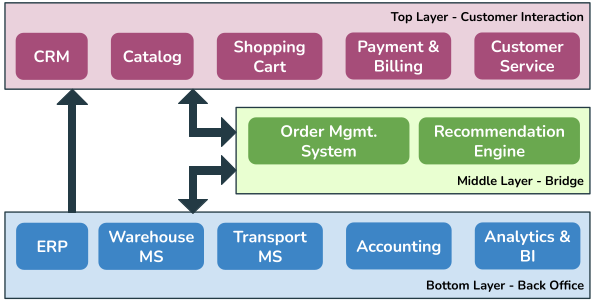
\includegraphics[scale=0.4]{01/crm.png}
    \caption{Esempio di e-commerce.}
\end{figure}

\paragraph{Commento dell'esempio:}

\begin{itemize}
  \item Ci sono tre livelli: 
    \begin{itemize}
      \item Top Layer: moduli che si rivolgono al cliente.
      \item Middle Layer: gestione della comunicazione tra cliente e azienda. 
      \item Bottom Layer: moduli interni aziendali.
    \end{itemize}
\end{itemize}

\paragraph{Requisiti non funzionali:}

\begin{itemize}
  \item High availability/zero downtime: l'applicativo deve essere sempre o quasi sempre disponibile. 
  \item Affidabilità: in caso di interruzione di workflow si deve far sì che non ci siano stati danni (e.g. un'interruzione durante una transazione). 
  \item Consistenza dei dati. 
  \item Integrità dei dati. 
  \item Low latency: per avere una buona performance, tutto deve essere fluido. 
  \item Scalabilità.
  \item Sicurezza. 
  \item Resilienza: capacità di reagire agli errori. 
  \item Mantenibilità: quanto un pezzo di software sia mantenibile o riutilizzabile.
  \item Osservabilità: per comprendere eventuali problemi in un sistema distribuito. 
  \item Auditability: le verifiche di qualità fatte su software\footnote{Meglio visto in "Etica, Società e Privacy".}.
\end{itemize}

\subsection{Panoramica Storica}

\dfn{Waterfall}{
  Le metodologie a cascata\footnote{Viste a "Sviluppo delle Applicazioni Software".} sono metodologie in cui ci sono fasi ben distinte e separate tra loro.
}

\nt{È un modello prevedibile, ma lento a gestire i cambiamenti.}

\clm{}{}{
  \begin{itemize}
    \item Software on the shelf: una volta acquistato è proprio. 
    \item Software custom: prodotto su richiesta, ha bisogno di tutto un servizio di manutenzione. 
  \end{itemize}
}

\dfn{Lean}{
  Metodologie nate negli anni '50 alla Toyota, verranno applicate al software dagli anni '90. Si basa su tre principi: 
  \begin{itemize}
    \item Muda\footnote{JOJO'S Reference} (waste): si deve stare sui requisiti, non mettere troppe funzioni non necessarie. 
    \item Mura (unevenness): è necessaria consinstenza per aumentare la prevedibilità.  
    \item Muri (overburden): non sovraccaricare le persone o le macchine. Non progettare software utilizzando strumenti greedy di risorse.
  \end{itemize} 
}

\nt{Lo strumento fondamentale è il \fancyglitter{kanban}: la lavagna, per organizzare il lavoro.}

\dfn{Siloed}{
  Organizzazione aziendale a silos: si comunica poco e male. Ci sono 4 gruppi: 
  \begin{itemize}
    \item BA Team: relazioni con gli stakeholders, requisiti, specifiche, documentazione. 
    \item Dev Team: programma e fa un minimo di unit testing. 
    \item Test Team: testa e decide se il sistema è pronto. 
    \item Ops Team: si occupa del deployement.
  \end{itemize}
}

\nt{I vari team si parlano in maniera molto limitata.}

\dfn{Transaction Processing Monitor}{
  I TP monitor erano il primo esempio di soluzione middleware. Usata nei sistemi di mainframe erano: centralizzati, monolitici, mission critical, con accesso da vari terminali.
}

\cor{Middleware}{
  Software nel mezzo tra applicazioni e infrastrutture. Permette alle applicazioni di utilizzare le infrastrutture per farle comunicare tra di loro.
}

\paragraph{Obiettivi:}

\begin{itemize}
  \item Performance: si occupa di transazioni rispettando le proprietà ACID. 
  \item Scalabilità: se un programma crasha ne avvia un'altra istanza. 
  \item Affidabilità. 
  \item Consistenza dei dati.
\end{itemize}

\paragraph{Limiti:}

\begin{itemize}
  \item Proprietario. 
  \item Tight coupling. 
  \item Costosi. 
  \item Complessi.
\end{itemize}

\qs{}{Cosa rimane dei TP monitors?}

\begin{itemize}
  \item \fancyglitter{Gestione delle transazioni e coordinazione:}
    \begin{itemize}
      \item Soluzioni basate su 2PC (2 Phase Commit). 
      \item Le proprietà ACID, attualmente supportate internamente da molti database. 
      \item Proprietà BASE: 
        \begin{itemize}
          \item Basically: risposte basiche.
          \item Available: si accetta che si possa non avere il dato più aggiornato. 
          \item State: la consistenza potrebbe non essere rispettata.
          \item Eventually: prima o poi si riceverà il dato corretto.
        \end{itemize}
    \end{itemize}
  \item \fancyglitter{Pool di connessioni}. 
  \item \fancyglitter{Distribuzione del carico:}
    \begin{itemize}
      \item Le richieste vengono distribuite su varie istanze. 
      \item In caso di fallimento l'applicazione riparte.
    \end{itemize}
\end{itemize}

\dfn{Remote Procedure Call}{
  Si chiama una funzione da una macchina remota come se fosse locale. È indipendente dal linguaggio e a una struttura silos. RIchiede aggiunte sia nello sviluppo che a runtime.
}

\begin{figure}[h]
    \centering
    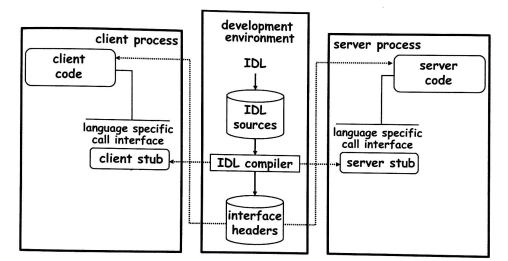
\includegraphics[scale=0.55]{01/rpc1.png}
    \caption{Remote Procedure Call - Development.}
\end{figure}

\begin{itemize}
  \item Serializzazione: trasformare i dati in qualcosa che può essere comunicato.
  \item Marshalling: usa la serializzazione e inserisce meta-dati per permettere la ricostruzione della struttura dati.
\end{itemize}

\begin{figure}[h]
    \centering
    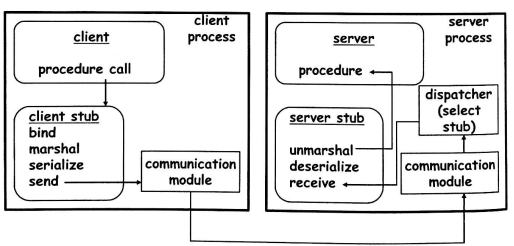
\includegraphics[scale=0.55]{01/rpc2.png}
    \caption{Remote Procedure Call - Runtime.}
\end{figure}

\dfn{Common Object Request Broker Architecture (CORBA)}{
  Evoluzione di rpc pensata per gli oggetti. Si possono creare oggetti in un server che possono rispondere a chiamate remote.
}

\nt{Più successo lo ha avuto RMI (Remote Method Invocation) che è CORBA, ma solo con Java.}

\paragraph{Limiti:}

\begin{itemize}
  \item Nascondere le cose al programmatore: si ha un falso senso di disaccoppiamento e i programmatori tendono a non vedere la rete. 
  \item La programmazione sembra semplice perché i problemi vengono sottovalutati.
\end{itemize}

\dfn{Message Oriented Middleware}{
  Invece di chiamarsi a vicenda le applicazioni si inviano messaggi a vicenda:
  \begin{itemize}
    \item Sincronizzazione tra operazioni in applicazioni diverse. 
    \item Notifiche di eventi. 
    \item Non c'è necessità di conoscere il ricevente.
  \end{itemize}
}

\paragraph{Due modelli di comunicazione:}

\begin{itemize}
  \item Point-to-Point: il mittente manda un messaggio nella coda del middleware, il ricevente lo consuma. 
  \item Publish and Subscribe: c'è una bacheca su cui chiunque può pubblicare un evento.
\end{itemize}

\dfn{Enterprise Service Bus (ESB)}{
  Un middleware coscente della logica di business. Si occupa di tradurre protocolli e dati.
}

\nt{Caduto totalmente in disuso.}

\dfn{AGILE}{
  Metodologie fondate su itertività e incrementalità.
}

\cor{XP - Xtreme Programming}{
  Si concentra sul codice, lo sviluppo di software si fa in team. Si dà importanza ai feedback sia dai clienti che dagli sviluppatori (small release, test-driven development, on-site customer).
}

\paragraph{Principi di XP:}

\begin{itemize}
  \item Comunicazione. 
  \item Semplicità. 
  \item Feedback. 
  \item Coraggio. 
  \item Rispetto.
\end{itemize}
